% Options for packages loaded elsewhere
\PassOptionsToPackage{unicode}{hyperref}
\PassOptionsToPackage{hyphens}{url}
\PassOptionsToPackage{dvipsnames,svgnames,x11names}{xcolor}
%
\documentclass[
  a4paper,
  DIV=11,
  numbers=noendperiod]{scrartcl}

\usepackage{amsmath,amssymb}
\usepackage{iftex}
\ifPDFTeX
  \usepackage[T1]{fontenc}
  \usepackage[utf8]{inputenc}
  \usepackage{textcomp} % provide euro and other symbols
\else % if luatex or xetex
  \usepackage{unicode-math}
  \defaultfontfeatures{Scale=MatchLowercase}
  \defaultfontfeatures[\rmfamily]{Ligatures=TeX,Scale=1}
\fi
\usepackage{lmodern}
\ifPDFTeX\else  
    % xetex/luatex font selection
\fi
% Use upquote if available, for straight quotes in verbatim environments
\IfFileExists{upquote.sty}{\usepackage{upquote}}{}
\IfFileExists{microtype.sty}{% use microtype if available
  \usepackage[]{microtype}
  \UseMicrotypeSet[protrusion]{basicmath} % disable protrusion for tt fonts
}{}
\makeatletter
\@ifundefined{KOMAClassName}{% if non-KOMA class
  \IfFileExists{parskip.sty}{%
    \usepackage{parskip}
  }{% else
    \setlength{\parindent}{0pt}
    \setlength{\parskip}{6pt plus 2pt minus 1pt}}
}{% if KOMA class
  \KOMAoptions{parskip=half}}
\makeatother
\usepackage{xcolor}
\setlength{\emergencystretch}{3em} % prevent overfull lines
\setcounter{secnumdepth}{5}
% Make \paragraph and \subparagraph free-standing
\makeatletter
\ifx\paragraph\undefined\else
  \let\oldparagraph\paragraph
  \renewcommand{\paragraph}{
    \@ifstar
      \xxxParagraphStar
      \xxxParagraphNoStar
  }
  \newcommand{\xxxParagraphStar}[1]{\oldparagraph*{#1}\mbox{}}
  \newcommand{\xxxParagraphNoStar}[1]{\oldparagraph{#1}\mbox{}}
\fi
\ifx\subparagraph\undefined\else
  \let\oldsubparagraph\subparagraph
  \renewcommand{\subparagraph}{
    \@ifstar
      \xxxSubParagraphStar
      \xxxSubParagraphNoStar
  }
  \newcommand{\xxxSubParagraphStar}[1]{\oldsubparagraph*{#1}\mbox{}}
  \newcommand{\xxxSubParagraphNoStar}[1]{\oldsubparagraph{#1}\mbox{}}
\fi
\makeatother


\providecommand{\tightlist}{%
  \setlength{\itemsep}{0pt}\setlength{\parskip}{0pt}}\usepackage{longtable,booktabs,array}
\usepackage{calc} % for calculating minipage widths
% Correct order of tables after \paragraph or \subparagraph
\usepackage{etoolbox}
\makeatletter
\patchcmd\longtable{\par}{\if@noskipsec\mbox{}\fi\par}{}{}
\makeatother
% Allow footnotes in longtable head/foot
\IfFileExists{footnotehyper.sty}{\usepackage{footnotehyper}}{\usepackage{footnote}}
\makesavenoteenv{longtable}
\usepackage{graphicx}
\makeatletter
\newsavebox\pandoc@box
\newcommand*\pandocbounded[1]{% scales image to fit in text height/width
  \sbox\pandoc@box{#1}%
  \Gscale@div\@tempa{\textheight}{\dimexpr\ht\pandoc@box+\dp\pandoc@box\relax}%
  \Gscale@div\@tempb{\linewidth}{\wd\pandoc@box}%
  \ifdim\@tempb\p@<\@tempa\p@\let\@tempa\@tempb\fi% select the smaller of both
  \ifdim\@tempa\p@<\p@\scalebox{\@tempa}{\usebox\pandoc@box}%
  \else\usebox{\pandoc@box}%
  \fi%
}
% Set default figure placement to htbp
\def\fps@figure{htbp}
\makeatother

\usepackage{booktabs}
\usepackage{caption}
\usepackage{longtable}
\usepackage{colortbl}
\usepackage{array}
\usepackage{anyfontsize}
\usepackage{multirow}
\KOMAoption{captions}{tableheading}
\makeatletter
\@ifpackageloaded{caption}{}{\usepackage{caption}}
\AtBeginDocument{%
\ifdefined\contentsname
  \renewcommand*\contentsname{Inhaltsverzeichnis}
\else
  \newcommand\contentsname{Inhaltsverzeichnis}
\fi
\ifdefined\listfigurename
  \renewcommand*\listfigurename{Abbildungsverzeichnis}
\else
  \newcommand\listfigurename{Abbildungsverzeichnis}
\fi
\ifdefined\listtablename
  \renewcommand*\listtablename{Tabellenverzeichnis}
\else
  \newcommand\listtablename{Tabellenverzeichnis}
\fi
\ifdefined\figurename
  \renewcommand*\figurename{Abbildung}
\else
  \newcommand\figurename{Abbildung}
\fi
\ifdefined\tablename
  \renewcommand*\tablename{Tabelle}
\else
  \newcommand\tablename{Tabelle}
\fi
}
\@ifpackageloaded{float}{}{\usepackage{float}}
\floatstyle{ruled}
\@ifundefined{c@chapter}{\newfloat{codelisting}{h}{lop}}{\newfloat{codelisting}{h}{lop}[chapter]}
\floatname{codelisting}{Listing}
\newcommand*\listoflistings{\listof{codelisting}{Listingverzeichnis}}
\makeatother
\makeatletter
\makeatother
\makeatletter
\@ifpackageloaded{caption}{}{\usepackage{caption}}
\@ifpackageloaded{subcaption}{}{\usepackage{subcaption}}
\makeatother

\ifLuaTeX
\usepackage[bidi=basic]{babel}
\else
\usepackage[bidi=default]{babel}
\fi
\babelprovide[main,import]{nswissgerman}
% get rid of language-specific shorthands (see #6817):
\let\LanguageShortHands\languageshorthands
\def\languageshorthands#1{}
\ifLuaTeX
  \usepackage[german]{selnolig} % disable illegal ligatures
\fi
\usepackage{bookmark}

\IfFileExists{xurl.sty}{\usepackage{xurl}}{} % add URL line breaks if available
\urlstyle{same} % disable monospaced font for URLs
\hypersetup{
  pdftitle={Tidycomm-tests},
  pdfauthor={Test Bär},
  pdflang={de-CH},
  colorlinks=true,
  linkcolor={blue},
  filecolor={Maroon},
  citecolor={Blue},
  urlcolor={Blue},
  pdfcreator={LaTeX via pandoc}}


\title{Tidycomm-tests}
\author{Test Bär}
\date{}

\begin{document}
\maketitle

\renewcommand*\contentsname{Inhaltsverzeichnis}
{
\hypersetup{linkcolor=}
\setcounter{tocdepth}{3}
\tableofcontents
}

\section{Regressionsanalyse mit den Daten ``World of
Journalism''}\label{regressionsanalyse-mit-den-daten-world-of-journalism}

Es ist immer ratsam sich zunächst die Regressionskoeffizienten genau
anzuschauen, was mit einer Tabelle praktisch am besten geht, wie sie in
Tabelle~\ref{tbl-tab1} einsehbar ist.

\begin{table}

\caption{\label{tbl-tab1}Regression auf autonome Auswahl}

\centering{

\fontsize{12.0pt}{14.4pt}\selectfont
\begin{tabular*}{0.85\linewidth}{@{\extracolsep{\fill}}lrrrrrrr}
\toprule
 & \multicolumn{4}{c}{unstd.} & std. & \multicolumn{2}{c}{sig.} \\ 
\cmidrule(lr){2-5} \cmidrule(lr){6-6} \cmidrule(lr){7-8}
Variable & B & SE B & LL & UL & B* & t & p \\ 
\midrule\addlinespace[2.5pt]
(Intercept) & 3.66 & 0.13 & 3.41 & 3.90 & — & 29.01 & <.001 \\ 
work\_experience & 0.01 & 0.00 & 0.01 & 0.02 & .160 & 5.37 & <.001 \\ 
trust\_government & 0.04 & 0.03 & -0.01 & 0.09 & .040 & 1.50 & .130 \\ 
ethics\_1 & -0.04 & 0.03 & -0.09 & 0.01 & -.040 & -1.43 & .150 \\ 
ethics\_2 & 0.01 & 0.02 & -0.03 & 0.06 & .020 & 0.68 & .490 \\ 
ethics\_3 & 0.00 & 0.02 & -0.05 & 0.04 & -.000 & -0.06 & .950 \\ 
ethics\_4 & -0.03 & 0.02 & -0.07 & 0.01 & -.050 & -1.46 & .140 \\ 
\bottomrule
\end{tabular*}
\begin{minipage}{\linewidth}
Autonomy Selection, R² = .034\\
F(6,1177) = 7, p = < .001, CI-Level = 95\%\\
\end{minipage}

}

\end{table}%

\begin{center}
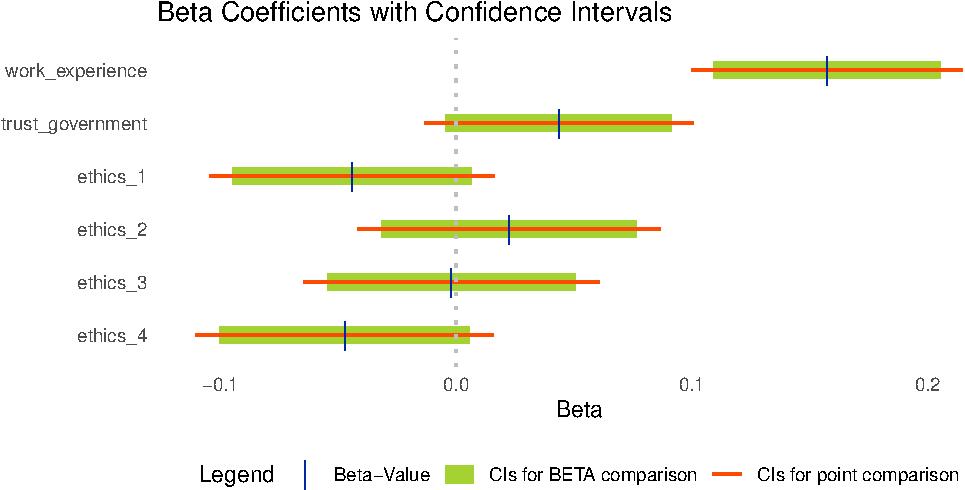
\includegraphics[width=0.85\linewidth,height=\textheight,keepaspectratio]{testthat_files/figure-pdf/unnamed-chunk-4-1.pdf}
\end{center}

\subsection{Teiltabelle}\label{teiltabelle}

\subsection{Analyse der
Voraussetzungen}\label{analyse-der-voraussetzungen}

In Abbildung~\ref{fig-reslev} ist gut zu erkennen.

\begin{figure}[H]

\centering{

\centering{

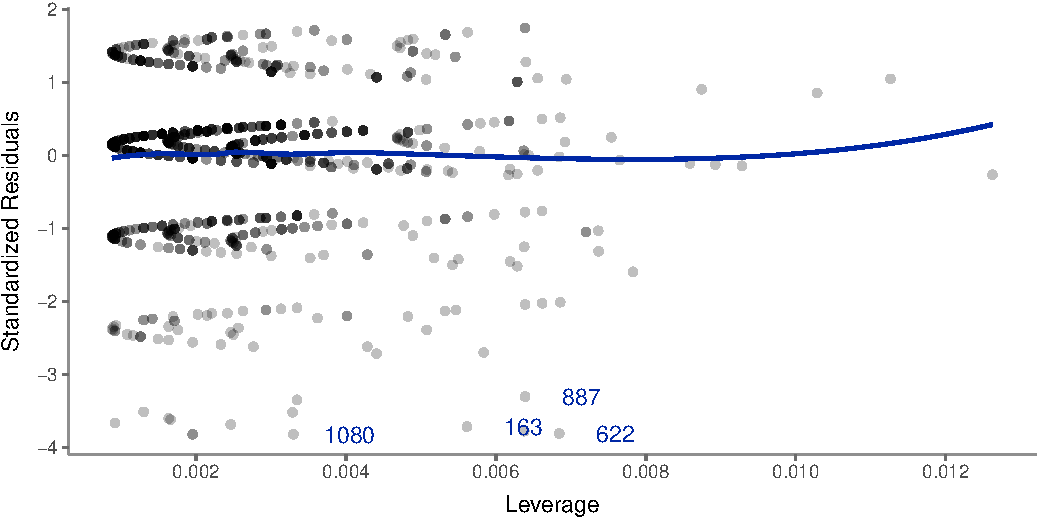
\includegraphics[width=0.85\linewidth,height=\textheight,keepaspectratio]{testthat_files/figure-pdf/fig-reslev-1.pdf}

}

\subcaption{\label{fig-reslev}}

}

\caption{\label{fig-reslev}residualsleverage plot}

\end{figure}%

Schaut man sich darüber hinaus Abbildung~\ref{fig-scaleloc} im schönen
UZH-Design an, wird einem alles klar.

\begin{figure}[H]

\centering{

\centering{

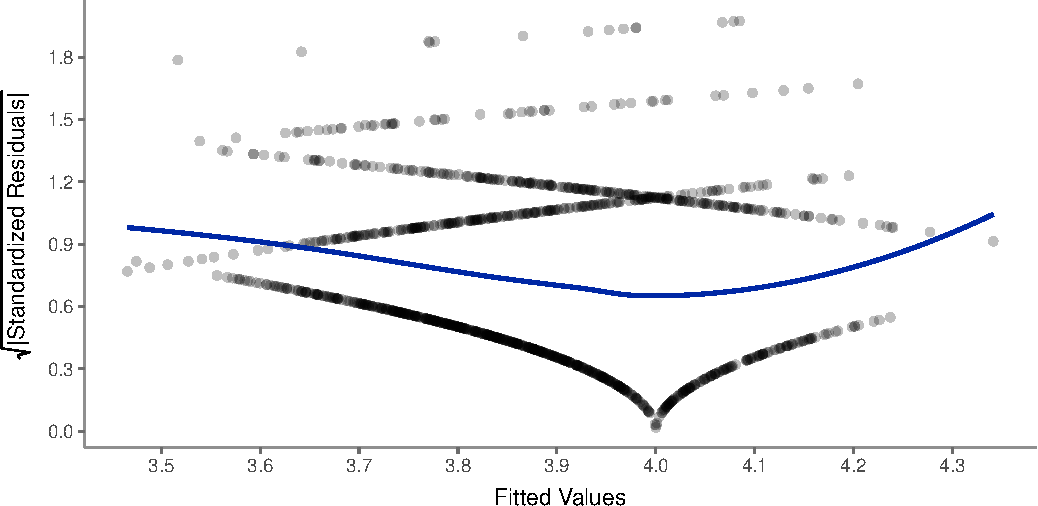
\includegraphics[width=0.85\linewidth,height=\textheight,keepaspectratio]{testthat_files/figure-pdf/fig-scaleloc-1.pdf}

}

\subcaption{\label{fig-scaleloc}}

}

\caption{\label{fig-scaleloc}scalelocation plot}

\end{figure}%

Nicht zuletzt sollte man sich die Residuen in Abhängigkeit der
geschätzten Werte ansehen, was im schönen Viridis-Design in
Abbildung~\ref{fig-resfit} durchaus möglich ist, auch wenn das dunkle
Lila nicht gut zu erkennen ist.

\begin{figure}[H]

\centering{

\centering{

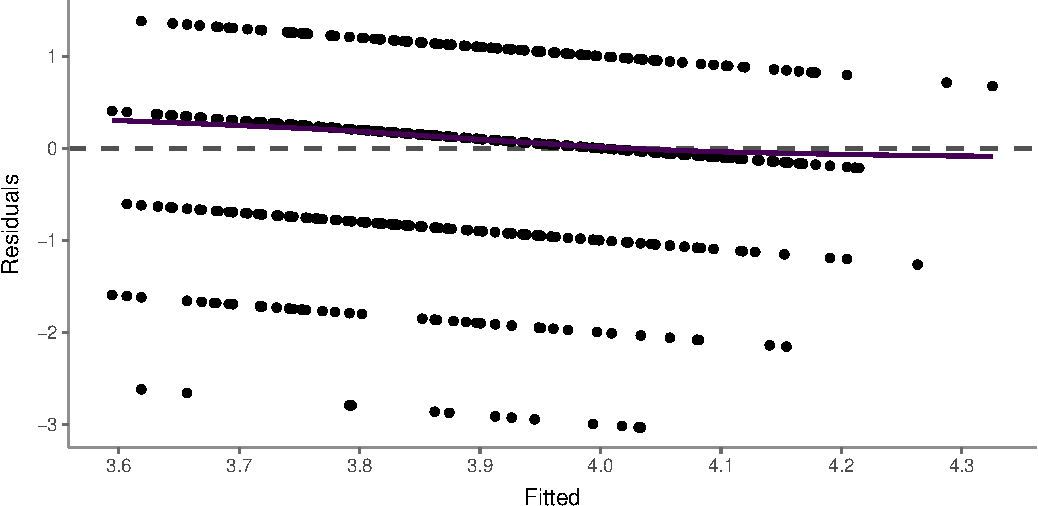
\includegraphics[width=0.85\linewidth,height=\textheight,keepaspectratio]{testthat_files/figure-pdf/fig-resfit-1.pdf}

}

\subcaption{\label{fig-resfit}}

}

\caption{\label{fig-resfit}residualsleverage plot}

\end{figure}%

\section{Häufigkeitsauszählung}\label{huxe4ufigkeitsauszuxe4hlung}

\begin{verbatim}
## <div id="lamgvuskem" style="padding-left:0px;padding-right:0px;padding-top:10px;padding-bottom:10px;overflow-x:auto;overflow-y:auto;width:auto;height:auto;">
##   <style>#lamgvuskem table {
##   font-family: system-ui, 'Segoe UI', Roboto, Helvetica, Arial, sans-serif, 'Apple Color Emoji', 'Segoe UI Emoji', 'Segoe UI Symbol', 'Noto Color Emoji';
##   -webkit-font-smoothing: antialiased;
##   -moz-osx-font-smoothing: grayscale;
## }
## 
## #lamgvuskem thead, #lamgvuskem tbody, #lamgvuskem tfoot, #lamgvuskem tr, #lamgvuskem td, #lamgvuskem th {
##   border-style: none;
## }
## 
## #lamgvuskem p {
##   margin: 0;
##   padding: 0;
## }
## 
## #lamgvuskem .gt_table {
##   display: table;
##   border-collapse: collapse;
##   line-height: normal;
##   margin-left: auto;
##   margin-right: auto;
##   color: #333333;
##   font-size: 16px;
##   font-weight: normal;
##   font-style: normal;
##   background-color: #FFFFFF;
##   width: 80%;
##   border-top-style: solid;
##   border-top-width: 2px;
##   border-top-color: #A8A8A8;
##   border-right-style: none;
##   border-right-width: 2px;
##   border-right-color: #D3D3D3;
##   border-bottom-style: solid;
##   border-bottom-width: 2px;
##   border-bottom-color: #A8A8A8;
##   border-left-style: none;
##   border-left-width: 2px;
##   border-left-color: #D3D3D3;
## }
## 
## #lamgvuskem .gt_caption {
##   padding-top: 4px;
##   padding-bottom: 4px;
## }
## 
## #lamgvuskem .gt_title {
##   color: #333333;
##   font-size: 125%;
##   font-weight: initial;
##   padding-top: 4px;
##   padding-bottom: 4px;
##   padding-left: 5px;
##   padding-right: 5px;
##   border-bottom-color: #FFFFFF;
##   border-bottom-width: 0;
## }
## 
## #lamgvuskem .gt_subtitle {
##   color: #333333;
##   font-size: 85%;
##   font-weight: initial;
##   padding-top: 3px;
##   padding-bottom: 5px;
##   padding-left: 5px;
##   padding-right: 5px;
##   border-top-color: #FFFFFF;
##   border-top-width: 0;
## }
## 
## #lamgvuskem .gt_heading {
##   background-color: #FFFFFF;
##   text-align: center;
##   border-bottom-color: #FFFFFF;
##   border-left-style: none;
##   border-left-width: 1px;
##   border-left-color: #D3D3D3;
##   border-right-style: none;
##   border-right-width: 1px;
##   border-right-color: #D3D3D3;
## }
## 
## #lamgvuskem .gt_bottom_border {
##   border-bottom-style: solid;
##   border-bottom-width: 2px;
##   border-bottom-color: #D3D3D3;
## }
## 
## #lamgvuskem .gt_col_headings {
##   border-top-style: solid;
##   border-top-width: 2px;
##   border-top-color: #D3D3D3;
##   border-bottom-style: solid;
##   border-bottom-width: 2px;
##   border-bottom-color: #D3D3D3;
##   border-left-style: none;
##   border-left-width: 1px;
##   border-left-color: #D3D3D3;
##   border-right-style: none;
##   border-right-width: 1px;
##   border-right-color: #D3D3D3;
## }
## 
## #lamgvuskem .gt_col_heading {
##   color: #333333;
##   background-color: #FFFFFF;
##   font-size: 100%;
##   font-weight: normal;
##   text-transform: inherit;
##   border-left-style: none;
##   border-left-width: 1px;
##   border-left-color: #D3D3D3;
##   border-right-style: none;
##   border-right-width: 1px;
##   border-right-color: #D3D3D3;
##   vertical-align: bottom;
##   padding-top: 5px;
##   padding-bottom: 6px;
##   padding-left: 5px;
##   padding-right: 5px;
##   overflow-x: hidden;
## }
## 
## #lamgvuskem .gt_column_spanner_outer {
##   color: #333333;
##   background-color: #FFFFFF;
##   font-size: 100%;
##   font-weight: normal;
##   text-transform: inherit;
##   padding-top: 0;
##   padding-bottom: 0;
##   padding-left: 4px;
##   padding-right: 4px;
## }
## 
## #lamgvuskem .gt_column_spanner_outer:first-child {
##   padding-left: 0;
## }
## 
## #lamgvuskem .gt_column_spanner_outer:last-child {
##   padding-right: 0;
## }
## 
## #lamgvuskem .gt_column_spanner {
##   border-bottom-style: solid;
##   border-bottom-width: 2px;
##   border-bottom-color: #D3D3D3;
##   vertical-align: bottom;
##   padding-top: 5px;
##   padding-bottom: 5px;
##   overflow-x: hidden;
##   display: inline-block;
##   width: 100%;
## }
## 
## #lamgvuskem .gt_spanner_row {
##   border-bottom-style: hidden;
## }
## 
## #lamgvuskem .gt_group_heading {
##   padding-top: 8px;
##   padding-bottom: 8px;
##   padding-left: 5px;
##   padding-right: 5px;
##   color: #333333;
##   background-color: #FFFFFF;
##   font-size: 100%;
##   font-weight: initial;
##   text-transform: inherit;
##   border-top-style: solid;
##   border-top-width: 2px;
##   border-top-color: #D3D3D3;
##   border-bottom-style: solid;
##   border-bottom-width: 2px;
##   border-bottom-color: #D3D3D3;
##   border-left-style: none;
##   border-left-width: 1px;
##   border-left-color: #D3D3D3;
##   border-right-style: none;
##   border-right-width: 1px;
##   border-right-color: #D3D3D3;
##   vertical-align: middle;
##   text-align: left;
## }
## 
## #lamgvuskem .gt_empty_group_heading {
##   padding: 0.5px;
##   color: #333333;
##   background-color: #FFFFFF;
##   font-size: 100%;
##   font-weight: initial;
##   border-top-style: solid;
##   border-top-width: 2px;
##   border-top-color: #D3D3D3;
##   border-bottom-style: solid;
##   border-bottom-width: 2px;
##   border-bottom-color: #D3D3D3;
##   vertical-align: middle;
## }
## 
## #lamgvuskem .gt_from_md > :first-child {
##   margin-top: 0;
## }
## 
## #lamgvuskem .gt_from_md > :last-child {
##   margin-bottom: 0;
## }
## 
## #lamgvuskem .gt_row {
##   padding-top: 8px;
##   padding-bottom: 8px;
##   padding-left: 5px;
##   padding-right: 5px;
##   margin: 10px;
##   border-top-style: solid;
##   border-top-width: 1px;
##   border-top-color: #D3D3D3;
##   border-left-style: none;
##   border-left-width: 1px;
##   border-left-color: #D3D3D3;
##   border-right-style: none;
##   border-right-width: 1px;
##   border-right-color: #D3D3D3;
##   vertical-align: middle;
##   overflow-x: hidden;
## }
## 
## #lamgvuskem .gt_stub {
##   color: #333333;
##   background-color: #FFFFFF;
##   font-size: 100%;
##   font-weight: initial;
##   text-transform: inherit;
##   border-right-style: solid;
##   border-right-width: 2px;
##   border-right-color: #D3D3D3;
##   padding-left: 5px;
##   padding-right: 5px;
## }
## 
## #lamgvuskem .gt_stub_row_group {
##   color: #333333;
##   background-color: #FFFFFF;
##   font-size: 100%;
##   font-weight: initial;
##   text-transform: inherit;
##   border-right-style: solid;
##   border-right-width: 2px;
##   border-right-color: #D3D3D3;
##   padding-left: 5px;
##   padding-right: 5px;
##   vertical-align: top;
## }
## 
## #lamgvuskem .gt_row_group_first td {
##   border-top-width: 2px;
## }
## 
## #lamgvuskem .gt_row_group_first th {
##   border-top-width: 2px;
## }
## 
## #lamgvuskem .gt_summary_row {
##   color: #333333;
##   background-color: #FFFFFF;
##   text-transform: inherit;
##   padding-top: 8px;
##   padding-bottom: 8px;
##   padding-left: 5px;
##   padding-right: 5px;
## }
## 
## #lamgvuskem .gt_first_summary_row {
##   border-top-style: solid;
##   border-top-color: #D3D3D3;
## }
## 
## #lamgvuskem .gt_first_summary_row.thick {
##   border-top-width: 2px;
## }
## 
## #lamgvuskem .gt_last_summary_row {
##   padding-top: 8px;
##   padding-bottom: 8px;
##   padding-left: 5px;
##   padding-right: 5px;
##   border-bottom-style: solid;
##   border-bottom-width: 2px;
##   border-bottom-color: #D3D3D3;
## }
## 
## #lamgvuskem .gt_grand_summary_row {
##   color: #333333;
##   background-color: #FFFFFF;
##   text-transform: inherit;
##   padding-top: 8px;
##   padding-bottom: 8px;
##   padding-left: 5px;
##   padding-right: 5px;
## }
## 
## #lamgvuskem .gt_first_grand_summary_row {
##   padding-top: 8px;
##   padding-bottom: 8px;
##   padding-left: 5px;
##   padding-right: 5px;
##   border-top-style: double;
##   border-top-width: 6px;
##   border-top-color: #D3D3D3;
## }
## 
## #lamgvuskem .gt_last_grand_summary_row_top {
##   padding-top: 8px;
##   padding-bottom: 8px;
##   padding-left: 5px;
##   padding-right: 5px;
##   border-bottom-style: double;
##   border-bottom-width: 6px;
##   border-bottom-color: #D3D3D3;
## }
## 
## #lamgvuskem .gt_striped {
##   background-color: rgba(128, 128, 128, 0.05);
## }
## 
## #lamgvuskem .gt_table_body {
##   border-top-style: solid;
##   border-top-width: 2px;
##   border-top-color: #D3D3D3;
##   border-bottom-style: solid;
##   border-bottom-width: 2px;
##   border-bottom-color: #D3D3D3;
## }
## 
## #lamgvuskem .gt_footnotes {
##   color: #333333;
##   background-color: #FFFFFF;
##   border-bottom-style: none;
##   border-bottom-width: 2px;
##   border-bottom-color: #D3D3D3;
##   border-left-style: none;
##   border-left-width: 2px;
##   border-left-color: #D3D3D3;
##   border-right-style: none;
##   border-right-width: 2px;
##   border-right-color: #D3D3D3;
## }
## 
## #lamgvuskem .gt_footnote {
##   margin: 0px;
##   font-size: 90%;
##   padding-top: 4px;
##   padding-bottom: 4px;
##   padding-left: 5px;
##   padding-right: 5px;
## }
## 
## #lamgvuskem .gt_sourcenotes {
##   color: #333333;
##   background-color: #FFFFFF;
##   border-bottom-style: none;
##   border-bottom-width: 2px;
##   border-bottom-color: #D3D3D3;
##   border-left-style: none;
##   border-left-width: 2px;
##   border-left-color: #D3D3D3;
##   border-right-style: none;
##   border-right-width: 2px;
##   border-right-color: #D3D3D3;
## }
## 
## #lamgvuskem .gt_sourcenote {
##   font-size: 90%;
##   padding-top: 4px;
##   padding-bottom: 4px;
##   padding-left: 5px;
##   padding-right: 5px;
## }
## 
## #lamgvuskem .gt_left {
##   text-align: left;
## }
## 
## #lamgvuskem .gt_center {
##   text-align: center;
## }
## 
## #lamgvuskem .gt_right {
##   text-align: right;
##   font-variant-numeric: tabular-nums;
## }
## 
## #lamgvuskem .gt_font_normal {
##   font-weight: normal;
## }
## 
## #lamgvuskem .gt_font_bold {
##   font-weight: bold;
## }
## 
## #lamgvuskem .gt_font_italic {
##   font-style: italic;
## }
## 
## #lamgvuskem .gt_super {
##   font-size: 65%;
## }
## 
## #lamgvuskem .gt_footnote_marks {
##   font-size: 75%;
##   vertical-align: 0.4em;
##   position: initial;
## }
## 
## #lamgvuskem .gt_asterisk {
##   font-size: 100%;
##   vertical-align: 0;
## }
## 
## #lamgvuskem .gt_indent_1 {
##   text-indent: 5px;
## }
## 
## #lamgvuskem .gt_indent_2 {
##   text-indent: 10px;
## }
## 
## #lamgvuskem .gt_indent_3 {
##   text-indent: 15px;
## }
## 
## #lamgvuskem .gt_indent_4 {
##   text-indent: 20px;
## }
## 
## #lamgvuskem .gt_indent_5 {
##   text-indent: 25px;
## }
## 
## #lamgvuskem .katex-display {
##   display: inline-flex !important;
##   margin-bottom: 0.75em !important;
## }
## 
## #lamgvuskem div.Reactable > div.rt-table > div.rt-thead > div.rt-tr.rt-tr-group-header > div.rt-th-group:after {
##   height: 0px !important;
## }
## </style>
##   <table class="gt_table" data-quarto-disable-processing="false" data-quarto-bootstrap="false">
##   <thead>
##     <tr class="gt_col_headings">
##       <th class="gt_col_heading gt_columns_bottom_border gt_left" rowspan="1" colspan="1" scope="col" id="autonomy_selection">autonomy_selection</th>
##       <th class="gt_col_heading gt_columns_bottom_border gt_right" rowspan="1" colspan="1" scope="col" id="N">N</th>
##       <th class="gt_col_heading gt_columns_bottom_border gt_right" rowspan="1" colspan="1" scope="col" id="Prozent">Prozent</th>
##       <th class="gt_col_heading gt_columns_bottom_border gt_right" rowspan="1" colspan="1" scope="col" id="Valide-%">Valide %</th>
##       <th class="gt_col_heading gt_columns_bottom_border gt_right" rowspan="1" colspan="1" scope="col" id="Kum-n">Kum n</th>
##       <th class="gt_col_heading gt_columns_bottom_border gt_right" rowspan="1" colspan="1" scope="col" id="Kum-%">Kum %</th>
##     </tr>
##   </thead>
##   <tbody class="gt_table_body">
##     <tr><td headers="autonomy_selection" class="gt_row gt_left">keine</td>
## <td headers="N" class="gt_row gt_right">14</td>
## <td headers="Prozent" class="gt_row gt_right">1%</td>
## <td headers="Valide %" class="gt_row gt_right">1%</td>
## <td headers="Kum n" class="gt_row gt_right">14</td>
## <td headers="Kum %" class="gt_row gt_right">1%</td></tr>
##     <tr><td headers="autonomy_selection" class="gt_row gt_left">2</td>
## <td headers="N" class="gt_row gt_right">50</td>
## <td headers="Prozent" class="gt_row gt_right">4%</td>
## <td headers="Valide %" class="gt_row gt_right">4%</td>
## <td headers="Kum n" class="gt_row gt_right">64</td>
## <td headers="Kum %" class="gt_row gt_right">5%</td></tr>
##     <tr><td headers="autonomy_selection" class="gt_row gt_left">3</td>
## <td headers="N" class="gt_row gt_right">235</td>
## <td headers="Prozent" class="gt_row gt_right">20%</td>
## <td headers="Valide %" class="gt_row gt_right">20%</td>
## <td headers="Kum n" class="gt_row gt_right">299</td>
## <td headers="Kum %" class="gt_row gt_right">25%</td></tr>
##     <tr><td headers="autonomy_selection" class="gt_row gt_left">4</td>
## <td headers="N" class="gt_row gt_right">670</td>
## <td headers="Prozent" class="gt_row gt_right">56%</td>
## <td headers="Valide %" class="gt_row gt_right">56%</td>
## <td headers="Kum n" class="gt_row gt_right">969</td>
## <td headers="Kum %" class="gt_row gt_right">81%</td></tr>
##     <tr><td headers="autonomy_selection" class="gt_row gt_left">volle</td>
## <td headers="N" class="gt_row gt_right">228</td>
## <td headers="Prozent" class="gt_row gt_right">19%</td>
## <td headers="Valide %" class="gt_row gt_right">19%</td>
## <td headers="Kum n" class="gt_row gt_right">1197</td>
## <td headers="Kum %" class="gt_row gt_right">100%</td></tr>
##     <tr><td headers="autonomy_selection" class="gt_row gt_left" style="color: #CCCCCC;">—</td>
## <td headers="N" class="gt_row gt_right" style="color: #CCCCCC;">3</td>
## <td headers="Prozent" class="gt_row gt_right" style="color: #CCCCCC;">0%</td>
## <td headers="Valide %" class="gt_row gt_right" style="color: #CCCCCC;">---</td>
## <td headers="Kum n" class="gt_row gt_right" style="color: #CCCCCC;">1200</td>
## <td headers="Kum %" class="gt_row gt_right" style="color: #CCCCCC;">---</td></tr>
##     <tr><td headers="autonomy_selection" class="gt_row gt_left">Gesamt</td>
## <td headers="N" class="gt_row gt_right">1200</td>
## <td headers="Prozent" class="gt_row gt_right">100%</td>
## <td headers="Valide %" class="gt_row gt_right">100%</td>
## <td headers="Kum n" class="gt_row gt_right">—</td>
## <td headers="Kum %" class="gt_row gt_right">—</td></tr>
##   </tbody>
##   
##   
## </table>
## </div>
## <div id="cfpkelyumi" style="padding-left:0px;padding-right:0px;padding-top:10px;padding-bottom:10px;overflow-x:auto;overflow-y:auto;width:auto;height:auto;">
##   <style>#cfpkelyumi table {
##   font-family: system-ui, 'Segoe UI', Roboto, Helvetica, Arial, sans-serif, 'Apple Color Emoji', 'Segoe UI Emoji', 'Segoe UI Symbol', 'Noto Color Emoji';
##   -webkit-font-smoothing: antialiased;
##   -moz-osx-font-smoothing: grayscale;
## }
## 
## #cfpkelyumi thead, #cfpkelyumi tbody, #cfpkelyumi tfoot, #cfpkelyumi tr, #cfpkelyumi td, #cfpkelyumi th {
##   border-style: none;
## }
## 
## #cfpkelyumi p {
##   margin: 0;
##   padding: 0;
## }
## 
## #cfpkelyumi .gt_table {
##   display: table;
##   border-collapse: collapse;
##   line-height: normal;
##   margin-left: auto;
##   margin-right: auto;
##   color: #333333;
##   font-size: 16px;
##   font-weight: normal;
##   font-style: normal;
##   background-color: #FFFFFF;
##   width: 80%;
##   border-top-style: solid;
##   border-top-width: 2px;
##   border-top-color: #A8A8A8;
##   border-right-style: none;
##   border-right-width: 2px;
##   border-right-color: #D3D3D3;
##   border-bottom-style: solid;
##   border-bottom-width: 2px;
##   border-bottom-color: #A8A8A8;
##   border-left-style: none;
##   border-left-width: 2px;
##   border-left-color: #D3D3D3;
## }
## 
## #cfpkelyumi .gt_caption {
##   padding-top: 4px;
##   padding-bottom: 4px;
## }
## 
## #cfpkelyumi .gt_title {
##   color: #333333;
##   font-size: 125%;
##   font-weight: initial;
##   padding-top: 4px;
##   padding-bottom: 4px;
##   padding-left: 5px;
##   padding-right: 5px;
##   border-bottom-color: #FFFFFF;
##   border-bottom-width: 0;
## }
## 
## #cfpkelyumi .gt_subtitle {
##   color: #333333;
##   font-size: 85%;
##   font-weight: initial;
##   padding-top: 3px;
##   padding-bottom: 5px;
##   padding-left: 5px;
##   padding-right: 5px;
##   border-top-color: #FFFFFF;
##   border-top-width: 0;
## }
## 
## #cfpkelyumi .gt_heading {
##   background-color: #FFFFFF;
##   text-align: center;
##   border-bottom-color: #FFFFFF;
##   border-left-style: none;
##   border-left-width: 1px;
##   border-left-color: #D3D3D3;
##   border-right-style: none;
##   border-right-width: 1px;
##   border-right-color: #D3D3D3;
## }
## 
## #cfpkelyumi .gt_bottom_border {
##   border-bottom-style: solid;
##   border-bottom-width: 2px;
##   border-bottom-color: #D3D3D3;
## }
## 
## #cfpkelyumi .gt_col_headings {
##   border-top-style: solid;
##   border-top-width: 2px;
##   border-top-color: #D3D3D3;
##   border-bottom-style: solid;
##   border-bottom-width: 2px;
##   border-bottom-color: #D3D3D3;
##   border-left-style: none;
##   border-left-width: 1px;
##   border-left-color: #D3D3D3;
##   border-right-style: none;
##   border-right-width: 1px;
##   border-right-color: #D3D3D3;
## }
## 
## #cfpkelyumi .gt_col_heading {
##   color: #333333;
##   background-color: #FFFFFF;
##   font-size: 100%;
##   font-weight: normal;
##   text-transform: inherit;
##   border-left-style: none;
##   border-left-width: 1px;
##   border-left-color: #D3D3D3;
##   border-right-style: none;
##   border-right-width: 1px;
##   border-right-color: #D3D3D3;
##   vertical-align: bottom;
##   padding-top: 5px;
##   padding-bottom: 6px;
##   padding-left: 5px;
##   padding-right: 5px;
##   overflow-x: hidden;
## }
## 
## #cfpkelyumi .gt_column_spanner_outer {
##   color: #333333;
##   background-color: #FFFFFF;
##   font-size: 100%;
##   font-weight: normal;
##   text-transform: inherit;
##   padding-top: 0;
##   padding-bottom: 0;
##   padding-left: 4px;
##   padding-right: 4px;
## }
## 
## #cfpkelyumi .gt_column_spanner_outer:first-child {
##   padding-left: 0;
## }
## 
## #cfpkelyumi .gt_column_spanner_outer:last-child {
##   padding-right: 0;
## }
## 
## #cfpkelyumi .gt_column_spanner {
##   border-bottom-style: solid;
##   border-bottom-width: 2px;
##   border-bottom-color: #D3D3D3;
##   vertical-align: bottom;
##   padding-top: 5px;
##   padding-bottom: 5px;
##   overflow-x: hidden;
##   display: inline-block;
##   width: 100%;
## }
## 
## #cfpkelyumi .gt_spanner_row {
##   border-bottom-style: hidden;
## }
## 
## #cfpkelyumi .gt_group_heading {
##   padding-top: 8px;
##   padding-bottom: 8px;
##   padding-left: 5px;
##   padding-right: 5px;
##   color: #333333;
##   background-color: #FFFFFF;
##   font-size: 100%;
##   font-weight: initial;
##   text-transform: inherit;
##   border-top-style: solid;
##   border-top-width: 2px;
##   border-top-color: #D3D3D3;
##   border-bottom-style: solid;
##   border-bottom-width: 2px;
##   border-bottom-color: #D3D3D3;
##   border-left-style: none;
##   border-left-width: 1px;
##   border-left-color: #D3D3D3;
##   border-right-style: none;
##   border-right-width: 1px;
##   border-right-color: #D3D3D3;
##   vertical-align: middle;
##   text-align: left;
## }
## 
## #cfpkelyumi .gt_empty_group_heading {
##   padding: 0.5px;
##   color: #333333;
##   background-color: #FFFFFF;
##   font-size: 100%;
##   font-weight: initial;
##   border-top-style: solid;
##   border-top-width: 2px;
##   border-top-color: #D3D3D3;
##   border-bottom-style: solid;
##   border-bottom-width: 2px;
##   border-bottom-color: #D3D3D3;
##   vertical-align: middle;
## }
## 
## #cfpkelyumi .gt_from_md > :first-child {
##   margin-top: 0;
## }
## 
## #cfpkelyumi .gt_from_md > :last-child {
##   margin-bottom: 0;
## }
## 
## #cfpkelyumi .gt_row {
##   padding-top: 8px;
##   padding-bottom: 8px;
##   padding-left: 5px;
##   padding-right: 5px;
##   margin: 10px;
##   border-top-style: solid;
##   border-top-width: 1px;
##   border-top-color: #D3D3D3;
##   border-left-style: none;
##   border-left-width: 1px;
##   border-left-color: #D3D3D3;
##   border-right-style: none;
##   border-right-width: 1px;
##   border-right-color: #D3D3D3;
##   vertical-align: middle;
##   overflow-x: hidden;
## }
## 
## #cfpkelyumi .gt_stub {
##   color: #333333;
##   background-color: #FFFFFF;
##   font-size: 100%;
##   font-weight: initial;
##   text-transform: inherit;
##   border-right-style: solid;
##   border-right-width: 2px;
##   border-right-color: #D3D3D3;
##   padding-left: 5px;
##   padding-right: 5px;
## }
## 
## #cfpkelyumi .gt_stub_row_group {
##   color: #333333;
##   background-color: #FFFFFF;
##   font-size: 100%;
##   font-weight: initial;
##   text-transform: inherit;
##   border-right-style: solid;
##   border-right-width: 2px;
##   border-right-color: #D3D3D3;
##   padding-left: 5px;
##   padding-right: 5px;
##   vertical-align: top;
## }
## 
## #cfpkelyumi .gt_row_group_first td {
##   border-top-width: 2px;
## }
## 
## #cfpkelyumi .gt_row_group_first th {
##   border-top-width: 2px;
## }
## 
## #cfpkelyumi .gt_summary_row {
##   color: #333333;
##   background-color: #FFFFFF;
##   text-transform: inherit;
##   padding-top: 8px;
##   padding-bottom: 8px;
##   padding-left: 5px;
##   padding-right: 5px;
## }
## 
## #cfpkelyumi .gt_first_summary_row {
##   border-top-style: solid;
##   border-top-color: #D3D3D3;
## }
## 
## #cfpkelyumi .gt_first_summary_row.thick {
##   border-top-width: 2px;
## }
## 
## #cfpkelyumi .gt_last_summary_row {
##   padding-top: 8px;
##   padding-bottom: 8px;
##   padding-left: 5px;
##   padding-right: 5px;
##   border-bottom-style: solid;
##   border-bottom-width: 2px;
##   border-bottom-color: #D3D3D3;
## }
## 
## #cfpkelyumi .gt_grand_summary_row {
##   color: #333333;
##   background-color: #FFFFFF;
##   text-transform: inherit;
##   padding-top: 8px;
##   padding-bottom: 8px;
##   padding-left: 5px;
##   padding-right: 5px;
## }
## 
## #cfpkelyumi .gt_first_grand_summary_row {
##   padding-top: 8px;
##   padding-bottom: 8px;
##   padding-left: 5px;
##   padding-right: 5px;
##   border-top-style: double;
##   border-top-width: 6px;
##   border-top-color: #D3D3D3;
## }
## 
## #cfpkelyumi .gt_last_grand_summary_row_top {
##   padding-top: 8px;
##   padding-bottom: 8px;
##   padding-left: 5px;
##   padding-right: 5px;
##   border-bottom-style: double;
##   border-bottom-width: 6px;
##   border-bottom-color: #D3D3D3;
## }
## 
## #cfpkelyumi .gt_striped {
##   background-color: rgba(128, 128, 128, 0.05);
## }
## 
## #cfpkelyumi .gt_table_body {
##   border-top-style: solid;
##   border-top-width: 2px;
##   border-top-color: #D3D3D3;
##   border-bottom-style: solid;
##   border-bottom-width: 2px;
##   border-bottom-color: #D3D3D3;
## }
## 
## #cfpkelyumi .gt_footnotes {
##   color: #333333;
##   background-color: #FFFFFF;
##   border-bottom-style: none;
##   border-bottom-width: 2px;
##   border-bottom-color: #D3D3D3;
##   border-left-style: none;
##   border-left-width: 2px;
##   border-left-color: #D3D3D3;
##   border-right-style: none;
##   border-right-width: 2px;
##   border-right-color: #D3D3D3;
## }
## 
## #cfpkelyumi .gt_footnote {
##   margin: 0px;
##   font-size: 90%;
##   padding-top: 4px;
##   padding-bottom: 4px;
##   padding-left: 5px;
##   padding-right: 5px;
## }
## 
## #cfpkelyumi .gt_sourcenotes {
##   color: #333333;
##   background-color: #FFFFFF;
##   border-bottom-style: none;
##   border-bottom-width: 2px;
##   border-bottom-color: #D3D3D3;
##   border-left-style: none;
##   border-left-width: 2px;
##   border-left-color: #D3D3D3;
##   border-right-style: none;
##   border-right-width: 2px;
##   border-right-color: #D3D3D3;
## }
## 
## #cfpkelyumi .gt_sourcenote {
##   font-size: 90%;
##   padding-top: 4px;
##   padding-bottom: 4px;
##   padding-left: 5px;
##   padding-right: 5px;
## }
## 
## #cfpkelyumi .gt_left {
##   text-align: left;
## }
## 
## #cfpkelyumi .gt_center {
##   text-align: center;
## }
## 
## #cfpkelyumi .gt_right {
##   text-align: right;
##   font-variant-numeric: tabular-nums;
## }
## 
## #cfpkelyumi .gt_font_normal {
##   font-weight: normal;
## }
## 
## #cfpkelyumi .gt_font_bold {
##   font-weight: bold;
## }
## 
## #cfpkelyumi .gt_font_italic {
##   font-style: italic;
## }
## 
## #cfpkelyumi .gt_super {
##   font-size: 65%;
## }
## 
## #cfpkelyumi .gt_footnote_marks {
##   font-size: 75%;
##   vertical-align: 0.4em;
##   position: initial;
## }
## 
## #cfpkelyumi .gt_asterisk {
##   font-size: 100%;
##   vertical-align: 0;
## }
## 
## #cfpkelyumi .gt_indent_1 {
##   text-indent: 5px;
## }
## 
## #cfpkelyumi .gt_indent_2 {
##   text-indent: 10px;
## }
## 
## #cfpkelyumi .gt_indent_3 {
##   text-indent: 15px;
## }
## 
## #cfpkelyumi .gt_indent_4 {
##   text-indent: 20px;
## }
## 
## #cfpkelyumi .gt_indent_5 {
##   text-indent: 25px;
## }
## 
## #cfpkelyumi .katex-display {
##   display: inline-flex !important;
##   margin-bottom: 0.75em !important;
## }
## 
## #cfpkelyumi div.Reactable > div.rt-table > div.rt-thead > div.rt-tr.rt-tr-group-header > div.rt-th-group:after {
##   height: 0px !important;
## }
## </style>
##   <table class="gt_table" data-quarto-disable-processing="false" data-quarto-bootstrap="false">
##   <thead>
##     <tr class="gt_col_headings">
##       <th class="gt_col_heading gt_columns_bottom_border gt_left" rowspan="1" colspan="1" scope="col" id="work_experience">work_experience</th>
##       <th class="gt_col_heading gt_columns_bottom_border gt_right" rowspan="1" colspan="1" scope="col" id="N">N</th>
##       <th class="gt_col_heading gt_columns_bottom_border gt_right" rowspan="1" colspan="1" scope="col" id="Prozent">Prozent</th>
##       <th class="gt_col_heading gt_columns_bottom_border gt_right" rowspan="1" colspan="1" scope="col" id="Valide-%">Valide %</th>
##       <th class="gt_col_heading gt_columns_bottom_border gt_right" rowspan="1" colspan="1" scope="col" id="Kum-n">Kum n</th>
##       <th class="gt_col_heading gt_columns_bottom_border gt_right" rowspan="1" colspan="1" scope="col" id="Kum-%">Kum %</th>
##     </tr>
##   </thead>
##   <tbody class="gt_table_body">
##     <tr><td headers="work_experience" class="gt_row gt_left">1</td>
## <td headers="N" class="gt_row gt_right">21</td>
## <td headers="Prozent" class="gt_row gt_right">2%</td>
## <td headers="Valide %" class="gt_row gt_right">2%</td>
## <td headers="Kum n" class="gt_row gt_right">21</td>
## <td headers="Kum %" class="gt_row gt_right">2%</td></tr>
##     <tr><td headers="work_experience" class="gt_row gt_left">2</td>
## <td headers="N" class="gt_row gt_right">33</td>
## <td headers="Prozent" class="gt_row gt_right">3%</td>
## <td headers="Valide %" class="gt_row gt_right">3%</td>
## <td headers="Kum n" class="gt_row gt_right">54</td>
## <td headers="Kum %" class="gt_row gt_right">5%</td></tr>
##     <tr><td headers="work_experience" class="gt_row gt_left">3</td>
## <td headers="N" class="gt_row gt_right">39</td>
## <td headers="Prozent" class="gt_row gt_right">3%</td>
## <td headers="Valide %" class="gt_row gt_right">3%</td>
## <td headers="Kum n" class="gt_row gt_right">93</td>
## <td headers="Kum %" class="gt_row gt_right">8%</td></tr>
##     <tr><td headers="work_experience" class="gt_row gt_left">4</td>
## <td headers="N" class="gt_row gt_right">46</td>
## <td headers="Prozent" class="gt_row gt_right">4%</td>
## <td headers="Valide %" class="gt_row gt_right">4%</td>
## <td headers="Kum n" class="gt_row gt_right">139</td>
## <td headers="Kum %" class="gt_row gt_right">12%</td></tr>
##     <tr><td headers="work_experience" class="gt_row gt_left">5</td>
## <td headers="N" class="gt_row gt_right">56</td>
## <td headers="Prozent" class="gt_row gt_right">5%</td>
## <td headers="Valide %" class="gt_row gt_right">5%</td>
## <td headers="Kum n" class="gt_row gt_right">195</td>
## <td headers="Kum %" class="gt_row gt_right">16%</td></tr>
##     <tr><td headers="work_experience" class="gt_row gt_left">6</td>
## <td headers="N" class="gt_row gt_right">19</td>
## <td headers="Prozent" class="gt_row gt_right">2%</td>
## <td headers="Valide %" class="gt_row gt_right">2%</td>
## <td headers="Kum n" class="gt_row gt_right">214</td>
## <td headers="Kum %" class="gt_row gt_right">18%</td></tr>
##     <tr><td headers="work_experience" class="gt_row gt_left">7</td>
## <td headers="N" class="gt_row gt_right">37</td>
## <td headers="Prozent" class="gt_row gt_right">3%</td>
## <td headers="Valide %" class="gt_row gt_right">3%</td>
## <td headers="Kum n" class="gt_row gt_right">251</td>
## <td headers="Kum %" class="gt_row gt_right">21%</td></tr>
##     <tr><td headers="work_experience" class="gt_row gt_left">8</td>
## <td headers="N" class="gt_row gt_right">47</td>
## <td headers="Prozent" class="gt_row gt_right">4%</td>
## <td headers="Valide %" class="gt_row gt_right">4%</td>
## <td headers="Kum n" class="gt_row gt_right">298</td>
## <td headers="Kum %" class="gt_row gt_right">25%</td></tr>
##     <tr><td headers="work_experience" class="gt_row gt_left">9</td>
## <td headers="N" class="gt_row gt_right">23</td>
## <td headers="Prozent" class="gt_row gt_right">2%</td>
## <td headers="Valide %" class="gt_row gt_right">2%</td>
## <td headers="Kum n" class="gt_row gt_right">321</td>
## <td headers="Kum %" class="gt_row gt_right">27%</td></tr>
##     <tr><td headers="work_experience" class="gt_row gt_left">10</td>
## <td headers="N" class="gt_row gt_right">74</td>
## <td headers="Prozent" class="gt_row gt_right">6%</td>
## <td headers="Valide %" class="gt_row gt_right">6%</td>
## <td headers="Kum n" class="gt_row gt_right">395</td>
## <td headers="Kum %" class="gt_row gt_right">33%</td></tr>
##     <tr><td headers="work_experience" class="gt_row gt_left">11</td>
## <td headers="N" class="gt_row gt_right">16</td>
## <td headers="Prozent" class="gt_row gt_right">1%</td>
## <td headers="Valide %" class="gt_row gt_right">1%</td>
## <td headers="Kum n" class="gt_row gt_right">411</td>
## <td headers="Kum %" class="gt_row gt_right">35%</td></tr>
##     <tr><td headers="work_experience" class="gt_row gt_left">12</td>
## <td headers="N" class="gt_row gt_right">28</td>
## <td headers="Prozent" class="gt_row gt_right">2%</td>
## <td headers="Valide %" class="gt_row gt_right">2%</td>
## <td headers="Kum n" class="gt_row gt_right">439</td>
## <td headers="Kum %" class="gt_row gt_right">37%</td></tr>
##     <tr><td headers="work_experience" class="gt_row gt_left">13</td>
## <td headers="N" class="gt_row gt_right">28</td>
## <td headers="Prozent" class="gt_row gt_right">2%</td>
## <td headers="Valide %" class="gt_row gt_right">2%</td>
## <td headers="Kum n" class="gt_row gt_right">467</td>
## <td headers="Kum %" class="gt_row gt_right">39%</td></tr>
##     <tr><td headers="work_experience" class="gt_row gt_left">14</td>
## <td headers="N" class="gt_row gt_right">16</td>
## <td headers="Prozent" class="gt_row gt_right">1%</td>
## <td headers="Valide %" class="gt_row gt_right">1%</td>
## <td headers="Kum n" class="gt_row gt_right">483</td>
## <td headers="Kum %" class="gt_row gt_right">41%</td></tr>
##     <tr><td headers="work_experience" class="gt_row gt_left">15</td>
## <td headers="N" class="gt_row gt_right">69</td>
## <td headers="Prozent" class="gt_row gt_right">6%</td>
## <td headers="Valide %" class="gt_row gt_right">6%</td>
## <td headers="Kum n" class="gt_row gt_right">552</td>
## <td headers="Kum %" class="gt_row gt_right">47%</td></tr>
##     <tr><td headers="work_experience" class="gt_row gt_left">16</td>
## <td headers="N" class="gt_row gt_right">35</td>
## <td headers="Prozent" class="gt_row gt_right">3%</td>
## <td headers="Valide %" class="gt_row gt_right">3%</td>
## <td headers="Kum n" class="gt_row gt_right">587</td>
## <td headers="Kum %" class="gt_row gt_right">49%</td></tr>
##     <tr><td headers="work_experience" class="gt_row gt_left">17</td>
## <td headers="N" class="gt_row gt_right">34</td>
## <td headers="Prozent" class="gt_row gt_right">3%</td>
## <td headers="Valide %" class="gt_row gt_right">3%</td>
## <td headers="Kum n" class="gt_row gt_right">621</td>
## <td headers="Kum %" class="gt_row gt_right">52%</td></tr>
##     <tr><td headers="work_experience" class="gt_row gt_left">18</td>
## <td headers="N" class="gt_row gt_right">27</td>
## <td headers="Prozent" class="gt_row gt_right">2%</td>
## <td headers="Valide %" class="gt_row gt_right">2%</td>
## <td headers="Kum n" class="gt_row gt_right">648</td>
## <td headers="Kum %" class="gt_row gt_right">55%</td></tr>
##     <tr><td headers="work_experience" class="gt_row gt_left">19</td>
## <td headers="N" class="gt_row gt_right">24</td>
## <td headers="Prozent" class="gt_row gt_right">2%</td>
## <td headers="Valide %" class="gt_row gt_right">2%</td>
## <td headers="Kum n" class="gt_row gt_right">672</td>
## <td headers="Kum %" class="gt_row gt_right">57%</td></tr>
##     <tr><td headers="work_experience" class="gt_row gt_left">20</td>
## <td headers="N" class="gt_row gt_right">69</td>
## <td headers="Prozent" class="gt_row gt_right">6%</td>
## <td headers="Valide %" class="gt_row gt_right">6%</td>
## <td headers="Kum n" class="gt_row gt_right">741</td>
## <td headers="Kum %" class="gt_row gt_right">62%</td></tr>
##     <tr><td headers="work_experience" class="gt_row gt_left">21</td>
## <td headers="N" class="gt_row gt_right">23</td>
## <td headers="Prozent" class="gt_row gt_right">2%</td>
## <td headers="Valide %" class="gt_row gt_right">2%</td>
## <td headers="Kum n" class="gt_row gt_right">764</td>
## <td headers="Kum %" class="gt_row gt_right">64%</td></tr>
##     <tr><td headers="work_experience" class="gt_row gt_left">22</td>
## <td headers="N" class="gt_row gt_right">17</td>
## <td headers="Prozent" class="gt_row gt_right">1%</td>
## <td headers="Valide %" class="gt_row gt_right">1%</td>
## <td headers="Kum n" class="gt_row gt_right">781</td>
## <td headers="Kum %" class="gt_row gt_right">66%</td></tr>
##     <tr><td headers="work_experience" class="gt_row gt_left">23</td>
## <td headers="N" class="gt_row gt_right">29</td>
## <td headers="Prozent" class="gt_row gt_right">2%</td>
## <td headers="Valide %" class="gt_row gt_right">2%</td>
## <td headers="Kum n" class="gt_row gt_right">810</td>
## <td headers="Kum %" class="gt_row gt_right">68%</td></tr>
##     <tr><td headers="work_experience" class="gt_row gt_left">24</td>
## <td headers="N" class="gt_row gt_right">20</td>
## <td headers="Prozent" class="gt_row gt_right">2%</td>
## <td headers="Valide %" class="gt_row gt_right">2%</td>
## <td headers="Kum n" class="gt_row gt_right">830</td>
## <td headers="Kum %" class="gt_row gt_right">70%</td></tr>
##     <tr><td headers="work_experience" class="gt_row gt_left">25</td>
## <td headers="N" class="gt_row gt_right">64</td>
## <td headers="Prozent" class="gt_row gt_right">5%</td>
## <td headers="Valide %" class="gt_row gt_right">5%</td>
## <td headers="Kum n" class="gt_row gt_right">894</td>
## <td headers="Kum %" class="gt_row gt_right">75%</td></tr>
##     <tr><td headers="work_experience" class="gt_row gt_left">26</td>
## <td headers="N" class="gt_row gt_right">17</td>
## <td headers="Prozent" class="gt_row gt_right">1%</td>
## <td headers="Valide %" class="gt_row gt_right">1%</td>
## <td headers="Kum n" class="gt_row gt_right">911</td>
## <td headers="Kum %" class="gt_row gt_right">77%</td></tr>
##     <tr><td headers="work_experience" class="gt_row gt_left">27</td>
## <td headers="N" class="gt_row gt_right">29</td>
## <td headers="Prozent" class="gt_row gt_right">2%</td>
## <td headers="Valide %" class="gt_row gt_right">2%</td>
## <td headers="Kum n" class="gt_row gt_right">940</td>
## <td headers="Kum %" class="gt_row gt_right">79%</td></tr>
##     <tr><td headers="work_experience" class="gt_row gt_left">28</td>
## <td headers="N" class="gt_row gt_right">21</td>
## <td headers="Prozent" class="gt_row gt_right">2%</td>
## <td headers="Valide %" class="gt_row gt_right">2%</td>
## <td headers="Kum n" class="gt_row gt_right">961</td>
## <td headers="Kum %" class="gt_row gt_right">81%</td></tr>
##     <tr><td headers="work_experience" class="gt_row gt_left">29</td>
## <td headers="N" class="gt_row gt_right">18</td>
## <td headers="Prozent" class="gt_row gt_right">2%</td>
## <td headers="Valide %" class="gt_row gt_right">2%</td>
## <td headers="Kum n" class="gt_row gt_right">979</td>
## <td headers="Kum %" class="gt_row gt_right">82%</td></tr>
##     <tr><td headers="work_experience" class="gt_row gt_left">30</td>
## <td headers="N" class="gt_row gt_right">60</td>
## <td headers="Prozent" class="gt_row gt_right">5%</td>
## <td headers="Valide %" class="gt_row gt_right">5%</td>
## <td headers="Kum n" class="gt_row gt_right">1039</td>
## <td headers="Kum %" class="gt_row gt_right">88%</td></tr>
##     <tr><td headers="work_experience" class="gt_row gt_left">31</td>
## <td headers="N" class="gt_row gt_right">8</td>
## <td headers="Prozent" class="gt_row gt_right">1%</td>
## <td headers="Valide %" class="gt_row gt_right">1%</td>
## <td headers="Kum n" class="gt_row gt_right">1047</td>
## <td headers="Kum %" class="gt_row gt_right">88%</td></tr>
##     <tr><td headers="work_experience" class="gt_row gt_left">32</td>
## <td headers="N" class="gt_row gt_right">16</td>
## <td headers="Prozent" class="gt_row gt_right">1%</td>
## <td headers="Valide %" class="gt_row gt_right">1%</td>
## <td headers="Kum n" class="gt_row gt_right">1063</td>
## <td headers="Kum %" class="gt_row gt_right">90%</td></tr>
##     <tr><td headers="work_experience" class="gt_row gt_left">33</td>
## <td headers="N" class="gt_row gt_right">11</td>
## <td headers="Prozent" class="gt_row gt_right">1%</td>
## <td headers="Valide %" class="gt_row gt_right">1%</td>
## <td headers="Kum n" class="gt_row gt_right">1074</td>
## <td headers="Kum %" class="gt_row gt_right">90%</td></tr>
##     <tr><td headers="work_experience" class="gt_row gt_left">34</td>
## <td headers="N" class="gt_row gt_right">8</td>
## <td headers="Prozent" class="gt_row gt_right">1%</td>
## <td headers="Valide %" class="gt_row gt_right">1%</td>
## <td headers="Kum n" class="gt_row gt_right">1082</td>
## <td headers="Kum %" class="gt_row gt_right">91%</td></tr>
##     <tr><td headers="work_experience" class="gt_row gt_left">35</td>
## <td headers="N" class="gt_row gt_right">34</td>
## <td headers="Prozent" class="gt_row gt_right">3%</td>
## <td headers="Valide %" class="gt_row gt_right">3%</td>
## <td headers="Kum n" class="gt_row gt_right">1116</td>
## <td headers="Kum %" class="gt_row gt_right">94%</td></tr>
##     <tr><td headers="work_experience" class="gt_row gt_left">36</td>
## <td headers="N" class="gt_row gt_right">3</td>
## <td headers="Prozent" class="gt_row gt_right">0%</td>
## <td headers="Valide %" class="gt_row gt_right">0%</td>
## <td headers="Kum n" class="gt_row gt_right">1119</td>
## <td headers="Kum %" class="gt_row gt_right">94%</td></tr>
##     <tr><td headers="work_experience" class="gt_row gt_left">37</td>
## <td headers="N" class="gt_row gt_right">8</td>
## <td headers="Prozent" class="gt_row gt_right">1%</td>
## <td headers="Valide %" class="gt_row gt_right">1%</td>
## <td headers="Kum n" class="gt_row gt_right">1127</td>
## <td headers="Kum %" class="gt_row gt_right">95%</td></tr>
##     <tr><td headers="work_experience" class="gt_row gt_left">38</td>
## <td headers="N" class="gt_row gt_right">7</td>
## <td headers="Prozent" class="gt_row gt_right">1%</td>
## <td headers="Valide %" class="gt_row gt_right">1%</td>
## <td headers="Kum n" class="gt_row gt_right">1134</td>
## <td headers="Kum %" class="gt_row gt_right">96%</td></tr>
##     <tr><td headers="work_experience" class="gt_row gt_left">39</td>
## <td headers="N" class="gt_row gt_right">6</td>
## <td headers="Prozent" class="gt_row gt_right">0%</td>
## <td headers="Valide %" class="gt_row gt_right">1%</td>
## <td headers="Kum n" class="gt_row gt_right">1140</td>
## <td headers="Kum %" class="gt_row gt_right">96%</td></tr>
##     <tr><td headers="work_experience" class="gt_row gt_left">40</td>
## <td headers="N" class="gt_row gt_right">24</td>
## <td headers="Prozent" class="gt_row gt_right">2%</td>
## <td headers="Valide %" class="gt_row gt_right">2%</td>
## <td headers="Kum n" class="gt_row gt_right">1164</td>
## <td headers="Kum %" class="gt_row gt_right">98%</td></tr>
##     <tr><td headers="work_experience" class="gt_row gt_left">41</td>
## <td headers="N" class="gt_row gt_right">2</td>
## <td headers="Prozent" class="gt_row gt_right">0%</td>
## <td headers="Valide %" class="gt_row gt_right">0%</td>
## <td headers="Kum n" class="gt_row gt_right">1166</td>
## <td headers="Kum %" class="gt_row gt_right">98%</td></tr>
##     <tr><td headers="work_experience" class="gt_row gt_left">42</td>
## <td headers="N" class="gt_row gt_right">4</td>
## <td headers="Prozent" class="gt_row gt_right">0%</td>
## <td headers="Valide %" class="gt_row gt_right">0%</td>
## <td headers="Kum n" class="gt_row gt_right">1170</td>
## <td headers="Kum %" class="gt_row gt_right">99%</td></tr>
##     <tr><td headers="work_experience" class="gt_row gt_left">43</td>
## <td headers="N" class="gt_row gt_right">4</td>
## <td headers="Prozent" class="gt_row gt_right">0%</td>
## <td headers="Valide %" class="gt_row gt_right">0%</td>
## <td headers="Kum n" class="gt_row gt_right">1174</td>
## <td headers="Kum %" class="gt_row gt_right">99%</td></tr>
##     <tr><td headers="work_experience" class="gt_row gt_left">44</td>
## <td headers="N" class="gt_row gt_right">3</td>
## <td headers="Prozent" class="gt_row gt_right">0%</td>
## <td headers="Valide %" class="gt_row gt_right">0%</td>
## <td headers="Kum n" class="gt_row gt_right">1177</td>
## <td headers="Kum %" class="gt_row gt_right">99%</td></tr>
##     <tr><td headers="work_experience" class="gt_row gt_left">45</td>
## <td headers="N" class="gt_row gt_right">4</td>
## <td headers="Prozent" class="gt_row gt_right">0%</td>
## <td headers="Valide %" class="gt_row gt_right">0%</td>
## <td headers="Kum n" class="gt_row gt_right">1181</td>
## <td headers="Kum %" class="gt_row gt_right">99%</td></tr>
##     <tr><td headers="work_experience" class="gt_row gt_left">46</td>
## <td headers="N" class="gt_row gt_right">1</td>
## <td headers="Prozent" class="gt_row gt_right">0%</td>
## <td headers="Valide %" class="gt_row gt_right">0%</td>
## <td headers="Kum n" class="gt_row gt_right">1182</td>
## <td headers="Kum %" class="gt_row gt_right">100%</td></tr>
##     <tr><td headers="work_experience" class="gt_row gt_left">49</td>
## <td headers="N" class="gt_row gt_right">1</td>
## <td headers="Prozent" class="gt_row gt_right">0%</td>
## <td headers="Valide %" class="gt_row gt_right">0%</td>
## <td headers="Kum n" class="gt_row gt_right">1183</td>
## <td headers="Kum %" class="gt_row gt_right">100%</td></tr>
##     <tr><td headers="work_experience" class="gt_row gt_left">50</td>
## <td headers="N" class="gt_row gt_right">2</td>
## <td headers="Prozent" class="gt_row gt_right">0%</td>
## <td headers="Valide %" class="gt_row gt_right">0%</td>
## <td headers="Kum n" class="gt_row gt_right">1185</td>
## <td headers="Kum %" class="gt_row gt_right">100%</td></tr>
##     <tr><td headers="work_experience" class="gt_row gt_left">51</td>
## <td headers="N" class="gt_row gt_right">1</td>
## <td headers="Prozent" class="gt_row gt_right">0%</td>
## <td headers="Valide %" class="gt_row gt_right">0%</td>
## <td headers="Kum n" class="gt_row gt_right">1186</td>
## <td headers="Kum %" class="gt_row gt_right">100%</td></tr>
##     <tr><td headers="work_experience" class="gt_row gt_left">53</td>
## <td headers="N" class="gt_row gt_right">1</td>
## <td headers="Prozent" class="gt_row gt_right">0%</td>
## <td headers="Valide %" class="gt_row gt_right">0%</td>
## <td headers="Kum n" class="gt_row gt_right">1187</td>
## <td headers="Kum %" class="gt_row gt_right">100%</td></tr>
##     <tr><td headers="work_experience" class="gt_row gt_left" style="color: #CCCCCC;">—</td>
## <td headers="N" class="gt_row gt_right" style="color: #CCCCCC;">13</td>
## <td headers="Prozent" class="gt_row gt_right" style="color: #CCCCCC;">1%</td>
## <td headers="Valide %" class="gt_row gt_right" style="color: #CCCCCC;">---</td>
## <td headers="Kum n" class="gt_row gt_right" style="color: #CCCCCC;">1200</td>
## <td headers="Kum %" class="gt_row gt_right" style="color: #CCCCCC;">---</td></tr>
##     <tr><td headers="work_experience" class="gt_row gt_left">Gesamt</td>
## <td headers="N" class="gt_row gt_right">1200</td>
## <td headers="Prozent" class="gt_row gt_right">100%</td>
## <td headers="Valide %" class="gt_row gt_right">100%</td>
## <td headers="Kum n" class="gt_row gt_right">—</td>
## <td headers="Kum %" class="gt_row gt_right">—</td></tr>
##   </tbody>
##   
##   
## </table>
## </div>
\end{verbatim}

\begin{table}
\fontsize{12.0pt}{14.4pt}\selectfont
\begin{tabular*}{0.8\linewidth}{@{\extracolsep{\fill}}lrrrrr}
\toprule
autonomy\_selection & N & Prozent & Valide \% & Kum n & Kum \% \\ 
\midrule\addlinespace[2.5pt]
1 & 14 & 1\% & 1\% & 14 & 1\% \\ 
2 & 50 & 4\% & 4\% & 64 & 5\% \\ 
3 & 235 & 20\% & 20\% & 299 & 25\% \\ 
4 & 670 & 56\% & 56\% & 969 & 81\% \\ 
5 & 228 & 19\% & 19\% & 1197 & 100\% \\ 
{\textcolor[HTML]{CCCCCC}{—}} & {\textcolor[HTML]{CCCCCC}{3}} & {\textcolor[HTML]{CCCCCC}{0\%}} & {\textcolor[HTML]{CCCCCC}{---}} & {\textcolor[HTML]{CCCCCC}{1200}} & {\textcolor[HTML]{CCCCCC}{---}} \\ 
Gesamt & 1200 & 100\% & 100\% & — & — \\ 
\bottomrule
\end{tabular*}
\begin{minipage}{\linewidth}
{Erste Zeile mit etwas Text, der dann umgebrochen werden}\\
{muss, damit er in die Breite der Tabelle passt.}\\
\end{minipage}
\end{table}




\end{document}
